\documentclass[12pt]{article}

\usepackage[utf8]{inputenc}
\usepackage[T1]{fontenc}
\usepackage[francais]{babel}
\usepackage{graphicx}

\usepackage{makeidx}

\usepackage[top=2cm, bottom=2cm, left=2cm, right=2cm]{geometry}

\title{\textbf{Rapport d'analyses sanguines}}
\author{Christophe \bsc{Néraud}}
\date{05/01/2018}

\makeindex

\begin{document}

\maketitle

\tableofcontents


\section{Définitions}
Cette section définit les différents paramètres étudiés par l'analyse. Elle présente également les causes et conséquences d'une quantité anormale de l'un de ces paramètres dans le sang.

	\subsection{Hématologie}
\textbf{L'hématologie\index{hematologie@hématologie}} est l'étude du sang et de ses éventuelles pathologies. Une analyse sanguine a pour but de fournir \textbf{l'hémogramme}\index{hemogramme@hémogramme} de l'individu, ainsi que le nombre de plaquettes dans le sang.

L'hémogramme donne des informations sur les éléments contenus dans le sang. Les informations qui y sont recueillies sont présentées dans les sous-sections suivantes.

	\subsubsection{Hématies}\index{hematie@hématie}
		\paragraph{Anatomie}\mbox{~}
				
	Aussi appelés \textit{érythrocytes}\index{erythrocyte@érythrocyte} ou \textit{globules rouges}\index{globules rouges}, ce sont des cellules sanguines de couleur rouge indispensables à l'oxygénation de l'organisme. Leur but est de transporter le dioxygène $\mathrm O_2$ et le dioxyde de carbone $\mathrm{CO}_2$ dans le sang.
	
	Les hématies se déplacent facilement dans le sang grâce à leur forme particulière qui leur confère une grande élasticité et une bonne résistance. En effet, les globules rouges ont la forme d'un disque \textbf{biconcave} d'un diamètre d'environ $7$ $\mu m$. Elles ne possèdent pas de noyau.
	
	La couleur rouge des érythrocytes vient de la présence \textbf{d'hémoglobine}\index{hemoglobine@hémoglobine} dans leur structure. Ce composé est un pigment rouge, dont le rôle est de fixer le dioxygène afin de le transporter jusqu'aux différents tissus de l'organisme.
	
	Ces cellules sont créées dans la moelle osseuse, grâce au processus \textit{d'érythropoïèse}\index{erythropoiese@érythropoïèse}. Ce procédé permet la synthèse de \textbf{plusieurs centaines de milliards} de globules rouges par jour, c'est-à-dire entre $2$ et $3$ millions par seconde. Les hématies ont une durée de vie d'environ 120 jours. Ainsi, les érythrocytes en fin de vie sont en permanence renouvelés.
	
		\paragraph{Physiologie}\mbox{~}
		
	Les hématies permettent le transport du dioxygène dans le sang grâce à l'hémoglobine : sa capacité à fixer et à libérer le dioxygène permet d'alimenter tous les organes. Le dioxygène est recueilli au niveau des poumons. Ces cellules permettent également de fixer le dioxyde de carbone rejeté par les organes grâce à une enzyme appelée \textit{anhydrase carbonique}\index{anhydrase carbonique} présente à la surface des hématies. Ces dernières vont ensuite libérer le dioxyde de carbone dans les poumons, pour qu'il soit ensuite rejeté au cours de l'expiration.
	
		\paragraph{Pathologies}\mbox{~}
		
	Les pathologies les plus courantes des hématies affectent leur taille, leur forme et leur concentration dans le sang.
	
	Un taux anormalement \textbf{bas} en globules rouges est caractéristique d'une \textit{anémie}\index{anemie@anémie}. Les causes de cette maladie peuvent être :
	\begin{itemize}
	\item Une anémie \textit{ferriprive}\index{anemie@anémie!ferriprive} ou \textit{microcytaire}\index{anemie@anémie!microcytaire} : elle est causée par une alimentation pauvre en fer, qui conduit à la formation d'hématies de petite taille.
	\item Une anémie \textit{par carence en vitamines} ou \textit{macrocytaire}\index{anemie@anémie!macrocytaire} : elle est causée par une carence en vitamine B12, qui conduit à la formation d'hématies de grande taille.
	\item Une anémie \textit{hémorragique} \index{anemie@anémie!hemorragique@hémorragique}: elle résulte d'une perte de sang importante, qui conduit donc à un déficit en hématies.
	\item Une anémie \textit{hémolytique}\index{anemie@anémie!hemolytique@hémolytique} : elle est due à une destruction trop rapide des hématies.
	\item Une anémie \textit{aplasique}\index{anemie@anémie!aplasique} : elle est causée par une synthèse insuffisante en hématies.
	\end{itemize}
	Les deux premières anémies peuvent être facilement prévenues par un apport suffisant en fer ou en vitamine B12. D'autres formes d'anémies peuvent être traitées par des médicaments ou compléments alimentaires. Dans les cas les plus graves, une greffe de la moelle osseuse ou un transfusion sanguine peuvent être envisagées.
	
	Au contraire, un taux anormalement \textbf{élevé} en érythrocytes est caractéristique d'une \textit{polyglobulie}\index{polyglobulie}. Des globules rouges sont produits en quantités excessives, et ce à cause d'agressions internes ou externes, ou lors de certaines maladies (par exemple la maladie de Vaquez). Le risque lié à cette maladie est la formation d'un caillot sanguin, on parle alors de \textbf{thrombose}.
	
	Une polyglobulie peut provenir également d'une \textit{hypoxie}\index{polyglobulie} : les tissus sont insuffisamment oxygénés, et il y a en conséquence augmentation du taux d'hormone stimulant l'érythropoïèse. Cette maladie se traduit par des céphalées, des vertiges, des acouphènes et une coloration rouge de la peau. Elle peut provenir de pneumopathie, cardiopathie congénitale, consommation excessive d'alcool ou de tabac, séjour en haute altitude ou encore port de vêtements trop serrés.
	
	Une autre pathologie importante des hématies est la \textit{drépanocytose}\index{drepanocytose@drépanocytose}. C'est une maladie génétique rare qui provoque des anomalies morphologiques des hématies : elles ont une forme de faucille. Elle peut être traitée par greffe de moelle osseuse ou transfusion sanguine.
	
		\paragraph{Valeurs de référence :} Dans un organisme en bonne santé, la quantité d'hématies moyenne se situe entre $4,28$ et $6,00$ Téra$/$L.
		
	\subsubsection{Hémoglobine}\index{hemoglobine@hémoglobine}
	L'hémoglobine est une \textit{métalloprotéine} contenant du fer. Elle est présente dans le sang, au sein des globules rouges. Sa fonction est de transporter l'oxygène $\mathrm O_2$ depuis les poumons jusqu'aux organes. Elle libère le dioxygène afin de permettre la respiration cellulaire aérobie \index{respiration cellulaire aerobie@respiration cellulaire aérobie}, qui fournit ensuite l'énergie nécessaire au fonctionnement des organes du corps.
	
		\paragraph{Structure}\mbox{~}
		
	L'hémoglobine est une protéine formée de chaînes peptidiques identiques deux à deux. Chez l'adulte, 95 \% de l'hémoglobine est de type A, notée HbA. Elle est constituée de deux chaînes $\alpha$ et de deux chaînes $\beta$. Il existe une hémoglobine A$_2$, notée HbA$_2$, composée de deux chaînes $\alpha$ et de deux chaînes $\delta$. Enfin, il existe une autre hémoglobine F, notée HbF, qui est fœtale et est composée de deux chaînes $\alpha$ et deux chaînes $\gamma$. Chacune de ces chaînes est associée à un groupe prosthétique appelé \textit{hème} et constitué d'un cation de fer complexé avec une porphyrine. Ainsi, l'hémoglobine est une \textit{homéoprotéine}.
	
		\paragraph{Synthèse}\mbox{~}
		
	L'hémoglobine est issue de l'érythropoïèse, elle est formée dans la moelle osseuse, comme les érythrocytes. L'hémoglobine ne se fixe sur les globules rouges qu'après la perte de leur noyau : il reste en effet de l'ARN messager dans la cellule, et celle-ci ne rentre en fonction que lorsqu'il a été éliminé.
	
		\paragraph{Pathologies}\mbox{~}
	
	Si le taux d'hémoglobine dans le sang est \textbf{faible}, il y a \textit{anémie}\index{anemie@anémie}. Elle est en général due à une carence en fer ou en vitamine B12, mais elle peut aussi être causée par une pathologie de la moelle osseuse, un cancer, le virus VIH, des pathologies gastro-intestinales et hépatiques, ou des maladies chroniques inflammatoires.
	
	Le taux d'hémoglobine dans le sang peut être \textbf{élevé} chez les personnes vivant à haute altitude. Elle peut aussi être causée par un \textit{emphysème}, ou la maladie de Vaquez.
	
		\paragraph{Valeurs de référence :} Dans un organisme en bonne santé, la quantité d'hémoglobine doit être comprise entre $13,0$ et $18,0$ g$/$dL, soit entre $8,1$ et $11,2$ mmol$/$L.
		
	\subsubsection{Hématocrite}\index{hematocrite@hématocrite}
	\textbf{L'hématocrite} correspond au volume occupé par les globules rouges dans le sang par rapport au volume total de sang, exprimé en pourcentage.
	
	C'est une donnée importante car elle permet de diagnostiquer des maladies telles que l'anémie\index{anemie@anémie}, la polyglobulie\index{polyglobulie} ou encore la déshydratation\index{deshydratation@déshydratation}. 
	
	L'hématocrite est directement lié à la quantité d'hématies mesurée lors d'une analyse de sang : sa diminution ou son élévation est causée par les mêmes pathologies que la diminution ou l'élévation de la quantité d'hématies dans le sang.
	
	Dans un organisme en bonne santé, l'hématocrite doit être compris entre $39,0$ et $53,0$ \%.
	
	\subsubsection{V.G.M.}\index{V.G.M.}
	Le \textbf{volume globulaire moyen}\index{volume globulaire moyen|see{V.G.M.}} (V.G.M.) est un paramètre qui caractérise la taille des hématies. Le V.G.M. est un indicateur très pratique pour détecter une anémie\index{anemie@anémie} : en effet, il permet de rendre compte d'une anémie microcytaire\index{anemie@anémie!microcytaire} ou macrocytaire\index{anemie@anémie!macrocytaire} car il donne accès à la taille des globules rouges, et donc permet de voir si ces cellules ont subi des anomalies structurelles.
	
	Une augmentation du V.G.M. peut résulter aussi bien d'une consommation excessive d'alcool que de maladies du foie.
	
	Dans un organisme en bonne santé, le V.G.M. doit se trouver entre $78,0$ et $98,0$ fL.
	
	\subsubsection{T.C.M.H.\index{T.C.M.H.} et C.C.M.H.\index{C.C.M.H.}}
	La \textbf{teneur corpusculaire moyenne en hémoglobine} (T.C.M.H.) et la \textbf{concentration corpusculaire moyenne en hémoglobine} (C.C.M.H.) sont deux indicateurs désignant respectivement la quantité moyenne d'hémoglobine se trouvant dans \textit{une} hématie et la quantité moyenne d'hémoglobine présente dans $100$ mL d'hématies.
	
	Dans un organisme en bonne santé, les valeurs de T.C.M.H. et de C.C.M.H. doivent être comprises entre respectivement $26,0$ et $34,0$ pg et entre $31,0$ et $36,5$ g$/$dL.
	
	\subsubsection{Index d'anisocytose}\index{anisocytose}
	L'anisocytose désigne une anomalie sanguine concernant la différence de taille entre plusieurs cellules sanguines, notamment les hématies et les plaquettes. On distingue l'anisocytose \textit{érythrocytaire}\index{anisocytose!erythrocytaire@érythrocytaire} lorsque l'anomalie concerne les globules rouges, et l'anisocytose \textit{plaquettaire}\index{anisocytose!plaquettaire} lorsqu'elle concerne les thrombocytes\index{thrombocyte}. On parle également \textbf{d'aniso-microcytose}\index{anisocytose!aniso-microcytose} lorsque les cellules sanguines sont anormalement petites, et \textbf{d'aniso-macrocytose}\index{anisocytose!aniso-macrocytose} lorsque les cellules sanguines sont anormalement grandes.
	
	Cette anomalie est généralement due à une anémie\index{anemie@anémie} ferriprive\index{anemie@anémie!ferriprive}, par carence en vitamines\index{anemie@anémie!macrocytaire} ou hémolytique\index{anemie@anémie!hemolytique@hémolytique}.
	
	Une anisocytose plaquettaire peut être due aux \textit{syndromes myélodysplasiques}\index{syndromes myelodysplasiques@syndromes myélodysplasiques} (SMD), qui sont des maladies de la moelle osseuse.
	
	\textit{L'index} d'anisocytose permet d'évaluer la variabilité de la taille des globules rouges au sein de la circulation sanguine, il détecte donc une anisocytose érythrocytaire.
	
	Dans un organisme en bonne santé, l'index d'anisocytose doit se trouver entre $10$ et $16$ \%.
	
	\subsubsection{Leucocytes}\index{leucocytes}
	Aussi appelés \textit{globules blancs}\index{globules blancs}, ce sont des cellules intervenant dans le système immunitaire.
	
		\paragraph{Anatomie}\mbox{~}
		
	Les leucocytes sont capables de circuler dans le sang, comme les hématies et les thrombocytes. Ils sont également présents dans le \textit{système lymphatique}\index{systeme lymphatique@système lymphatique} aussi appelé \textit{lymphe}\index{lymphe}, dans certains tissus conjonctifs et dans certains \textit{organes lymphoïdes}\index{organe lymphoide@organe lymphoïde} tels les ganglions ou la rate. Les leucocytes sont créés dans la moelle osseuse, comme les hématies.
	
	On peut classer les leucocytes en trois groupes :
	\begin{itemize}
	\item Les \textit{granulocytes}\index{granulocyte} : ils représentent entre $40$ et $80$\% des leucocytes de l'organisme. Ils regroupent les granulocytes \textit{neutrophiles}\index{granulocyte!neutrophile}, \textit{basophiles}\index{granulocyte!basophile} et \textit{éosinophiles}\index{granulocyte!eosinohpile@éosinophile}.
	\item Les \textit{lymphocytes}\index{lymphocytes} : ils représentent entre $20$ et $40$\% des leucocytes, et regroupent les lymphocytes \textit{B}\index{lymphocytes!B}, \textit{T}\index{lymphocytes!T} et les cellules \textit{Natural Killer}\index{lymphocytes!Natural Killer (NK)} (NK).
	\item Les \textit{monocytes}\index{monocyte} : ils représentent entre $2$ et $10$\% des leucocytes, et regroupent les \textit{macrophages}\index{monocyte!macrophage} et les \textit{cellules dendritiques}\index{monocyte!cellule dendritique}.
	\end{itemize}
	
		\paragraph{Physiologie}\mbox{~}
		
	Les leucocytes font partie des défenses de l'organisme. Elles interviennent notamment dans la \textit{réponse immunitaire innée}\index{reponse immunitaire innee@réponse immunitaire innée} et dans la \textit{réponse immunitaire adaptative}\index{reponse immunitaire adaptative@réponse immunitaire adaptative}.
	
	La réponse immunitaire innée est la première réaction de l'organisme lors d'une agression par des agents pathogènes. Elle se traduit notamment par une \textit{réaction inflammatoire}\index{reaction inflammatoire@réaction inflammatoire}. Ce mécanisme joue un rôle essentiel dans l'élimination des agents pathogènes. Il fait intervenir plusieurs globules blancs dont :
	\begin{itemize}
	\item \textbf{les macrophages} : ils jouent un rôle de phagocyte\index{phagocyte}, ces cellules sont en effet capables d'ingérer et de digérer les agents pathogènes ;
	\item \textbf{les cellules NK} : elles détruisent les cellules altérées, infectées ou tumorales ;
	\item \textbf{les éosinophiles} : elles luttent contrent les infections parasitaires ;
	\item \textbf{les basophiles} :  ils participent à la réponse inflammatoire ;
	\item \textbf{les cellules dendritiques} : elles permettent l'activation de la réponse immunitaire adaptative en transmettant les informations concernant l'agent pathogène aux organes lymphoïdes.
	\end{itemize}
	
	La réponse immunitaire adaptative est la suite de la réponse immunitaire innée. Au contraire de cette dernière, elle n'est pas immédiate mais est spécifique. Cette réaction est principalement basée sur la reconnaissance des agents pathogènes  : un agent pathogène infectant le corps est tout d'abord mémorisé lors de la réponse immunitaire innée, et peut être ensuite reconnu lors d'une autre agression. Ce système fait intervenir deux types de lymphocytes :
	\begin{itemize}
	\item \textbf{les lymphocytes T} : ils maintiennent active la réponse immunitaire et détruisent les agents pathogènes ;
	\item \textbf{les lymphocytes B} : ils produisent des anticorps, des protéines complexes qui ont la capacité de se fixer à l'agent pathogène afin de le neutraliser ; il est ensuite digéré par des macrophages.
	\end{itemize}
	
		\paragraph{Pathologie}\mbox{~}
		
	Les leucocytes peuvent souffrir de plusieurs pathologies telles qu'une maladie auto-immune, des allergies, le VIH, le cancer, etc.
	
	Dans le cas d'une maladie auto-immune\index{maladie auto-immune}, le système immunitaire fonctionne anormalement : les anticorps produits par les lymphocytes B attaquent les cellules de l'organisme. On peut citer par exemple la \textit{polyarthrite rhumatoïde}\index{polyarthrite rhumatoide@polyarthrite rhumatoïde}, la \textit{sclérose}\index{sclerose@sclérose} ou encore le \textit{diabète de type 1}\index{diabete@diabète}.
	
	Les réponses allergiques sont causées par une libération d'histamine par les granulocytes basophiles.
	
	Le \textbf{Virus d'Immunodéficience Humaine} (VIH)\index{VIH} est à l'origine du \textit{syndrome d'immunodéficience acquise} (SIDA)\index{SIDA}. Ce syndrome se caractérise par un affaiblissement général du système immunitaire, et rend l'organisme vulnérable à des maladies opportunistes.
	
	Certains \textbf{cancers}\index{cancer} peuvent également affecter les leucocytes, tels que :
	\begin{itemize}
	\item une \textit{leucémie}\index{leucemie@leucémie} : c'est un cancer des cellules de la moelle osseuse, ce qui perturbe donc la production des cellules sanguines ;
	\item un \textit{lymphome}\index{lymphome} : c'est un cancer du système lymphatique ;
	\item un \textit{myélome}\index{myelome@myélome} : c'est un cancer hématologique ;
	\item la \textit{maladie de Waldenström}\index{maladie de Waldenstrom@maladie de Waldenström} : c'est également un cancer hématologique.
	\end{itemize}
	
	Les leucocytes peuvent subir d'autres anomalies. Lors de l'établissement de l'hémogramme, une quantité trop faible de leucocytes correspond à une \textit{leucopénie}\index{leucopenie@leucopénie}. Un taux anormalement élevé de leucocytes correspond en revanche à une \textit{hyperleucocytose}\index{hyperleucocytose}.
	
	Un myélogramme permet également de quantifier la production de leucocytes par la moelle osseuse.
	
	Enfin, \textit{un examen cytobactériologique des urines} (ECBU)\index{ECBU} permet d'évaluer la quantité de leucocytes présents dans les urines. Un taux élevé de globules blancs dans les urines est révélateur d'une infection : c'est une \textit{leucocyturie}\index{leucocyturie}.
	
		\paragraph{Traitements et prévention}\mbox{~}
		
	L'infection par le VIH est évitable par l'usage d'une protection adéquate lors de rapports sexuels. Des traitements médicaux peuvent également être mis en place afin de traiter les pathologies des leucocytes : anti-histaminiques dans le cas d'allergies, traitements à base d'antirétroviraux pour le VIH. Il existe également des traitements nécessitant chimiotérapie ou radiothérapie.
	
	Dans certains cas sévères, on peut pratiquer une greffe de moelle osseuse. Cela est notamment nécessaire lors d'une leucémie.
	
		\paragraph{Valeurs de référence :}
	Dans un organisme en bonne santé, la quantité de leucocytes doit être comprise entre $4,0$ et $11,0$ Giga$/$L.
	
	\subsubsection{Plaquettes}\index{plaquette}
	Les plaquettes ont un rôle très important dans la coagulation\index{coagulation} du sang. Elles permettent entre autre d'arrêter les hémorragies.
	
	Un taux trop bas de plaquettes dans le sang augmente le risque d'hémorragies. Ceci peut être causé par des leucémies aiguës, les lymphomes, les métastases et la myélofibrose. 
	
	Lorsque le taux est trop élevé, il y a un fort risque de thrombose\index{thrombose} : formation d'un caillot sanguin. Ceci témoigne de maladies de la moelle osseuse, ou bien de :
	\begin{itemize}
	\item une maladie inflammatoire,
	\item une carence en fer,
	\item une asplénie et splenectomie,
	\item un cancer,
	\item un stress important,
	\item une dépression.
	\end{itemize}		
	
	Dans un organisme en bonne santé, la quantité de plaquettes doit être comprise entre $150$ et $400$ Giga$/$L.
	
	L'étude des plaquettes fait intervenir la mesure du V.P.M.\index{V.P.M.}, le \textit{volume plaquettaire moyen}\index{volume plaquettaire moyen|see{V.P.M.}}. Cette grandeur traduit le volume moyen des plaquettes. Les plaquettes jeunes étant plus grosses, une augmentation du V.P.M. exprime une augmentation du nombre de plaquettes produites. Dans un organisme en bonne santé, le V.P.M. ne doit pas dépasser $11,0$ fL.
	
	\subsection{Protéines Sériques}
	Les protéines sont les briques essentielles de nos cellules. Il existe une centaine de protéines différentes dans le sang. Toutefois, \textit{l'albumine}\index{albumine} représente $60\%$ d'entre elles. Les protéines jouent un rôle important car elles permettent d'une part de transporter de nombreuses substances telles que les hormones, les lipides, etc. D'autre part, les protéines du sang interviennent dans la coagulation\index{coagulation}, l'immunité, le maintien de la pression sanguine, etc.
	
	L'analyse des protéines sériques, c'est-à-dire les protéines présentes dans le sérum\index{serum@sérum}, permet d'évaluer le fonctionnement du foie et des reins, et de mettre en évidence certaines anomalies : syndrome inflammatoire, maladies auto-immunes, lymphomes, etc.
	
	L'analyse de ces protéines se fait par électrophorèse\index{electrophorese@électrophorèse} du sang : un champ électrique appliqué au sérum fait se déplacer les protéines. Elle se séparent et il est ainsi facile de les distinguer et de repérer des anomalies.
	
	Une augmentation des protéines plasmatiques totales, c'est-à-dire une \textit{hyperprotidémie}\index{hyperprotidemie@hyperprotidémie} est observée en cas de déshydratation ou au cours de maladies telles que le myélome.
	
	Une diminution de la concentration des protéines totales, c'est-à-dire une \textit{hypoprotidémie}\index{hypoprotidemie@hypoprotidémie}, est causée par un défaut d'apport (malnutrition) ou un défaut d'absorption, par un défaut de synthèse (insuffisance hépatique), par une perte anormale au niveau du rein ou encore de la surcharge hydrique (hémodilution).
	
		\subsubsection{Protéine C réactive}\index{proteine C reactive@protéine C réactive|see{CRP}}
	Aussi appelée CRP\index{CRP}, la protéine C réactive est une protéine synthétisée par le foie à la suite d'une inflammation de l'organisme. Normalement, elle disparaît dès l'éradication de l'agent infectieux de l'organisme.
	
	Lors d'une agression intérieure ou extérieure du corps par un agent pathogène ou une maladie, des messagers sont entre autres libérés dans le sang, ce sont les \textit{cytokines}\index{cytokine}. Le but de ses substances est de provoquer de multiples signaux clinico-biologiques ayant un effet sur le système nerveux (fièvre par exemple), les vaisseaux sanguins, mais également le fois qui va synthétiser les protéines de l'inflammation, dont la CRP.
	
	La protéine C réactive joue un rôle dans la réponse immunitaire. Elle permet en effet de mobiliser et d'activer les leucocytes, ainsi que de stimuler la phagocytose. Lors d'une agression, le taux de protéines C réactives peut être très rapidement multiplié par 1000.
	
	La réaction inflammatoire aiguë s'accompagne de rougeur, gonflement, sensation de chaleur et de douleur : ces éléments sont dus à la \textit{vasodilatation}\index{vasodilatation}. Elle peut être également à l'origine de fièvre, asthénie, troubles du sommeil et anorexie.
	
	Les pathologies susceptibles d'élever la concentration en CRP sont les suivantes :
	\begin{itemize}
	\item Les infections bactériennes.
	\item Les parasitoses et mycoses profondes.
	\item Les infections virales chroniques (VIH, hépatites\index{hepatite@hépatite} B et C).
	\item Les néoplasies (i.e. cancer profond ou avec métastases, lymphome hodgkinien et non hodgkinien, leucémies).
	\item Les pathologies systémiques et rhumatismales (polyarthrite rhumatoïde, spondylarthrite ankylosante, vascularite, maladie de Horton, maladie de Wegener, myosite, maladie de Still, lupus érythémateux).
	\item Les pathologies digestives (maladie de Crohn).
	\item Les nécroses ischémiques (infarctus).
	\item Les traumatismes (chirurgies, brûlures).
	\end{itemize}
	
	Il est nécessaire de contrôler la quantité de CRP dans l'organisme. En effet, une augmentation modérée et chronique du taux de protéine C réactive représenterait un facteur de risque demaladies cardiovasculaires. Les CRP pourraient également être un acteur direct de l'athérogenèse.
	
	Dans un organisme en bonne santé, la quantité de protéine C réactive doit être inférieure à $5$ mg$/$L, soit inférieure à $46$ nmol$/$L.
	
	\subsection{Enzymologie}\index{enzymologie}
	L'enzymologie est l'étude des \textbf{enzymes}\index{enzyme}. Elle comprend l'étude des réactions enzymatiques, s'appuyant sur la cinétique réactionnelle, ainsi que l'approche structurale des enzymes et leur relation avec leur activité : ceci permet notamment de classer les enzymes selon une nomenclature particulière.
	
	Une analyse de sang s'intéresse à quatre enzymes : les transaminases\index{transaminase} SGOT\index{transaminase!SGOT} et SGPT\index{transaminase!SGPT}, les gamma-glutamyl transférase et les phosphatases alcalines.
		
		\subsubsection{Transaminases}
	Les transaminases sont des enzymes présentes à l'intérieur des cellules, en particulier au niveau du foie et des muscles. On distingue les \textit{transaminases ASAT}\index{transaminase!ASAT|see{SGOT}} pour \textbf{aspartate aminotransférases}\index{aspartate aminotransferase@aspartate aminotransférase|see{ASAT}} qui sont surtout présentes dans le foie, les muscles, le coeur, les reins, le cerveau et le pancréas, des \textit{transminases ALAT}\index{transaminase!ALAT|see{SGPT}} pour \textbf{alanine aminotransférases}\index{alanine aminotransferase@alanine aminotransférase|see{ALAT}} qui sont relativement spécifiques au foie. Le sigle SGOT signifie \textit{sérum-glutamyl-oxaloacétate-transférase}\index{serum-glutamyl-oxaloacetate-transferase@sérum-glutamyl-oxaloacétate-transférase|see{SGOT}}, et le sigle SGPT signifie \textit{sérum-glutamyl-pyruvate-transférase}\index{serum-glutamyl-pyruvate-transferase@sérum-glutamyl-pyruvate-transférase|see{SGPT}}.
	
	Le dosage des transaminases permet de détecter un problème au niveau du foie : leur concentration dans le sang augmente à cause d'une libération anormale par des cellules hépatiques endommagées, par exemple en raison d'une hépatite\index{hepatite@hépatite}, d'une intoxication alcoolique ou médicamenteuse, etc. Les symptômes généraux d'une quantité anormale de transaminases dans le sang sont : fatigue, baisse de forme, nausées, ictère. 
	
	Des concentrations d'ASAT et d'ALAT anormalement élevées traduisent une atteinte hépatique. Une élévation légère (2-3 fois la norme) ou modérée (3-10 fois la norme) survient en cas de trouble hépatique lié à l'alcool, en cas d'hépatite\index{hepatite@hépatite} virale chronique ou de stéatose. Un rapport ASAT/ALAT supérieur à 2 traduit généralement une maladie alcoolique du foie. 
	
	En revanche, une élévation importante (supérieure à 10 à 20 fois la norme) correspond à une hépatite\index{hepatite@hépatite} virale aiguë, à des lésions induites par des médicaments ou une intoxication, ainsi qu'à une ischémie hépatique (i.e. un arrêt partiel de l'irrigation sanguine au niveau du foie).
	
	Dans un organisme en bonne santé, la quantité de transaminases SGOT doit être inférieure à $33$ U$/$L, et celle de transaminases SGPT à $26$ U$/$L, où U est l'unité enzymatique.
	
	\subsubsection{Gamma-glutamyl transférase}\index{gamma-glutamyl transferase@gamma-glutamyl transférase|see{gamma-GT}}
	Les gamma-glutamyl transférase ou gamma-glutamyl transpeptidase, aussi appelés \textit{gamma-GT}\index{gamma-GT}, sont des protéines produites par notamment les cellules du foie (les hépatocytes\index{hepatocyte@hépatocyte}). Les gamma-GT permettent la réalisation de réactions chimiques indispensables comme le transfert de certains acides aminés. En revanche, ces enzymes ne se transforment jamais et ne modifient aucun composant, il n'y a ainsi aucune conséquence \textit{directe} à leur augmentation ou leur diminution dans l'organisme. Ces éléments permettent néanmoins de souligner un dysfonctionnement.
	
	Le taux de gamma-GT est souvent plus élevé que la norme sans qu'il n'y ait de pathologie associée à cette augmentation, c'est souvent inexplicable. Des paramètres peuvent connus peuvent également faire s'élever le taux de gamma-GT, tels que : les maladies hépato-biliaires, l'hyperlipidémie, le diabète. Toutefois, les trois causes principales de l'augmentation de la quantité de gamma-GT sont :
	\begin{itemize}
	\item une surcharge pondérale,
	\item la prise de médicaments,
	\item l'alcoolisme chronique.
	\end{itemize}
	
	Dans un organisme en bonne santé, il est recommandé que la concentration en gamma-GT soit inférieure à $29$ U$/$L, mais cette norme est à relativiser.
	
	\subsubsection{Phosphatases alcalines}\index{phosphatase alcaline|see{PAL}}
	Aussi notées PAL\index{PAL}, les phosphatases alcalines sont des enzymes se trouvant dans la plupart des tissus de l'organisme, mais plus particulièrement dans les os, le fois, l'intestin, les reins. Elles sont également présentes dans le placenta lors de la grossesse. Le taux de PAL augmente naturellement pendant la croissance, mais son augmentation peut également refléter une maladie hépatique ou osseuse lorsqu'elle survient en dehors de la période de croissance.
	
	Le dosage des PAL permet de dépister une atteinte hépatique, mais également une \textit{cholestase}\index{cholestase} (i.e. l'arrêt ou la stagnation de l'écoulement de la bile dans les voies biliaires) et des obstructions biliaires.
	
	Le dosage des PAL nécessite d'être à jeun lors de la prise de sang. Une élévation des phosphatases alcalines est ainsi normale chez l'adolescent, la femme enceinte, mais peut traduire également une maladie du foie, ou encore une maladie osseuse telle que : la maladie de Paget, des métastases osseuses, une ostéomalacie, une fracture ou un tassement vertébral, etc.
	
	En revanche, une concentration basse en PAL indique un dysfonctionnement grave du foie : c'est une \textit{insuffisance hépatocellulaire}\index{insuffisance hepatocellulaire@insuffisance hépatocellulaire}, causée par une cirrhose\index{cirrhose} ou une hépatite\index{hepatite@hépatite}.
	
	Dans un organisme en bonne santé, la concentration en phosphatases alcalines doit être comprise entre $55$ et $149$ U$/$L.
	
	\subsection{Biochimie}
		\subsubsection{Glycémie à jeun}
	La glycémie\index{glycemie@glycémie} représente la quantité de glucose présente dans le sang. Sa mesure nécessite impérativement d'être à jeun, car l'alimentation du sujet peut modifier la quantité de glucose. Le fait d'être à jeun permet donc d'évaluer la glycémie << naturelle >> du patient. 
	
	L'étude de la glycémie permet de déceler des maladies telles que le diabète\index{diabete@diabète}. Dans un organisme en bonne santé, la glycémie doit être comprise entre $4,11$ et $5,89$ mmol$/$L, soit entre $0,74$ et $1,06$ g$/$L.
	
		\subsubsection{Aspect du sérum}
	Lors d'une analyse sanguine, l'aspect du sérum permet de déceler une dyslipidémie\index{dyslipidemie@dyslipidémie}. Ce paramètre est important pour détecter des maladies ou des risques de maladies cardiovasculaires.
	
	Dans un organisme en bonne santé, l'aspect du sérum doit être <<clair>> ou <<limpide>>.
	
		\subsubsection{Triglycérides}\index{triglyceride@triglycéride}
	Les triglycérides sont des graisses (lipides\index{lipide}) qui servent de réserve énergétique. Elles proviennent essentiellement de l'alimentation, mais sont aussi synthétisées par le foie. Elles constituent un risque cardiovasculaire car, en trop grande quantité dans le sang, elles peuvent boucher les artères.
	
	La mesure de la quantité de triglycérides permet de détecter des maladies telles que la dyslipidémie\index{dyslipidemie@dyslipidémie}, mais aussi le diabète\index{diabete@diabète} de type 2, une hypertension artérielle\index{hypertension}, etc.
	
	Dans un organisme en bonne santé, la concentration en triglycérides doit être inférieure à $1,70$ mmol$/$L, soit $1,50$ g$/$L. Une concentration supérieure à $4$ g$/$L constitue une \textit{hypertriglycéridémie}\index{hypertriglyceridemie@hypertriglycéridémie}.
	
	
	
	
	
	
	
\newpage
\section{Résultats d'analyse}
	\subsection{Analyses du 03 janvier 2018}
	\begin{figure}[!h]
		\begin{center}
		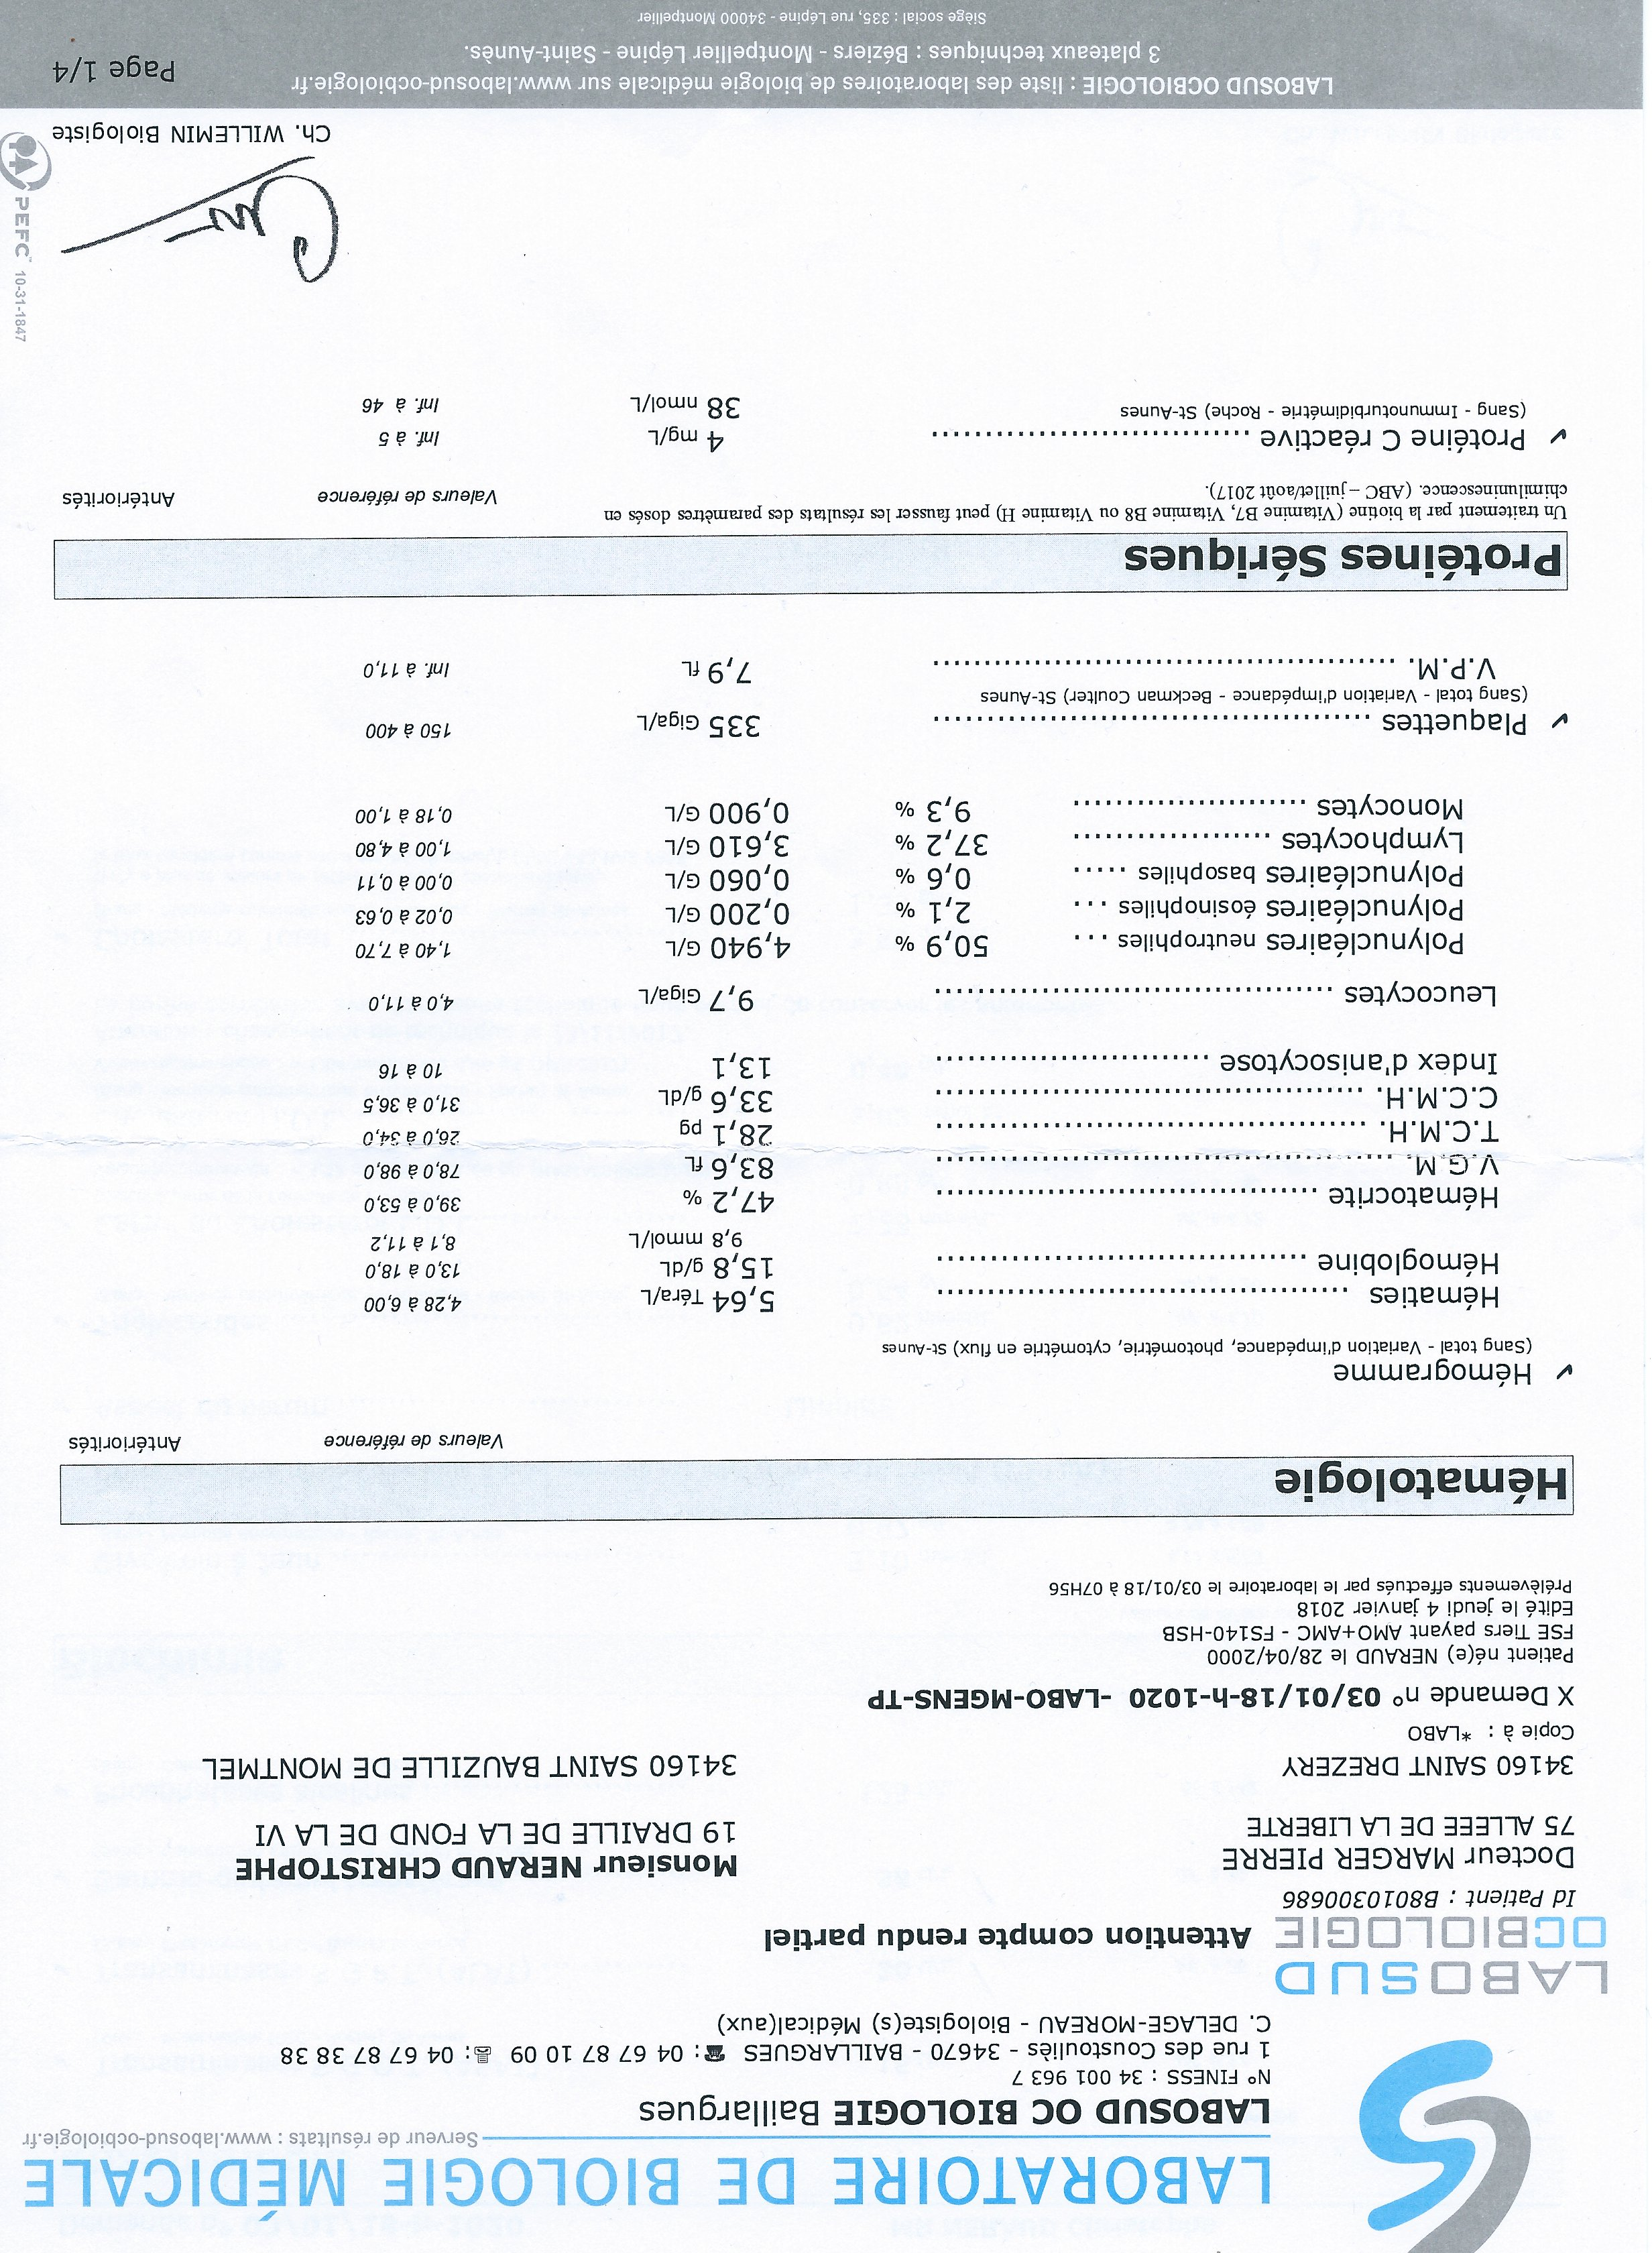
\includegraphics[angle=180, scale=0.71]{03-01-2018/p1.JPG}
		\end{center}
		\caption{03 janvier 2018 : page 1}
	\end{figure}
	
	\begin{figure}[!h]
		\begin{center}
		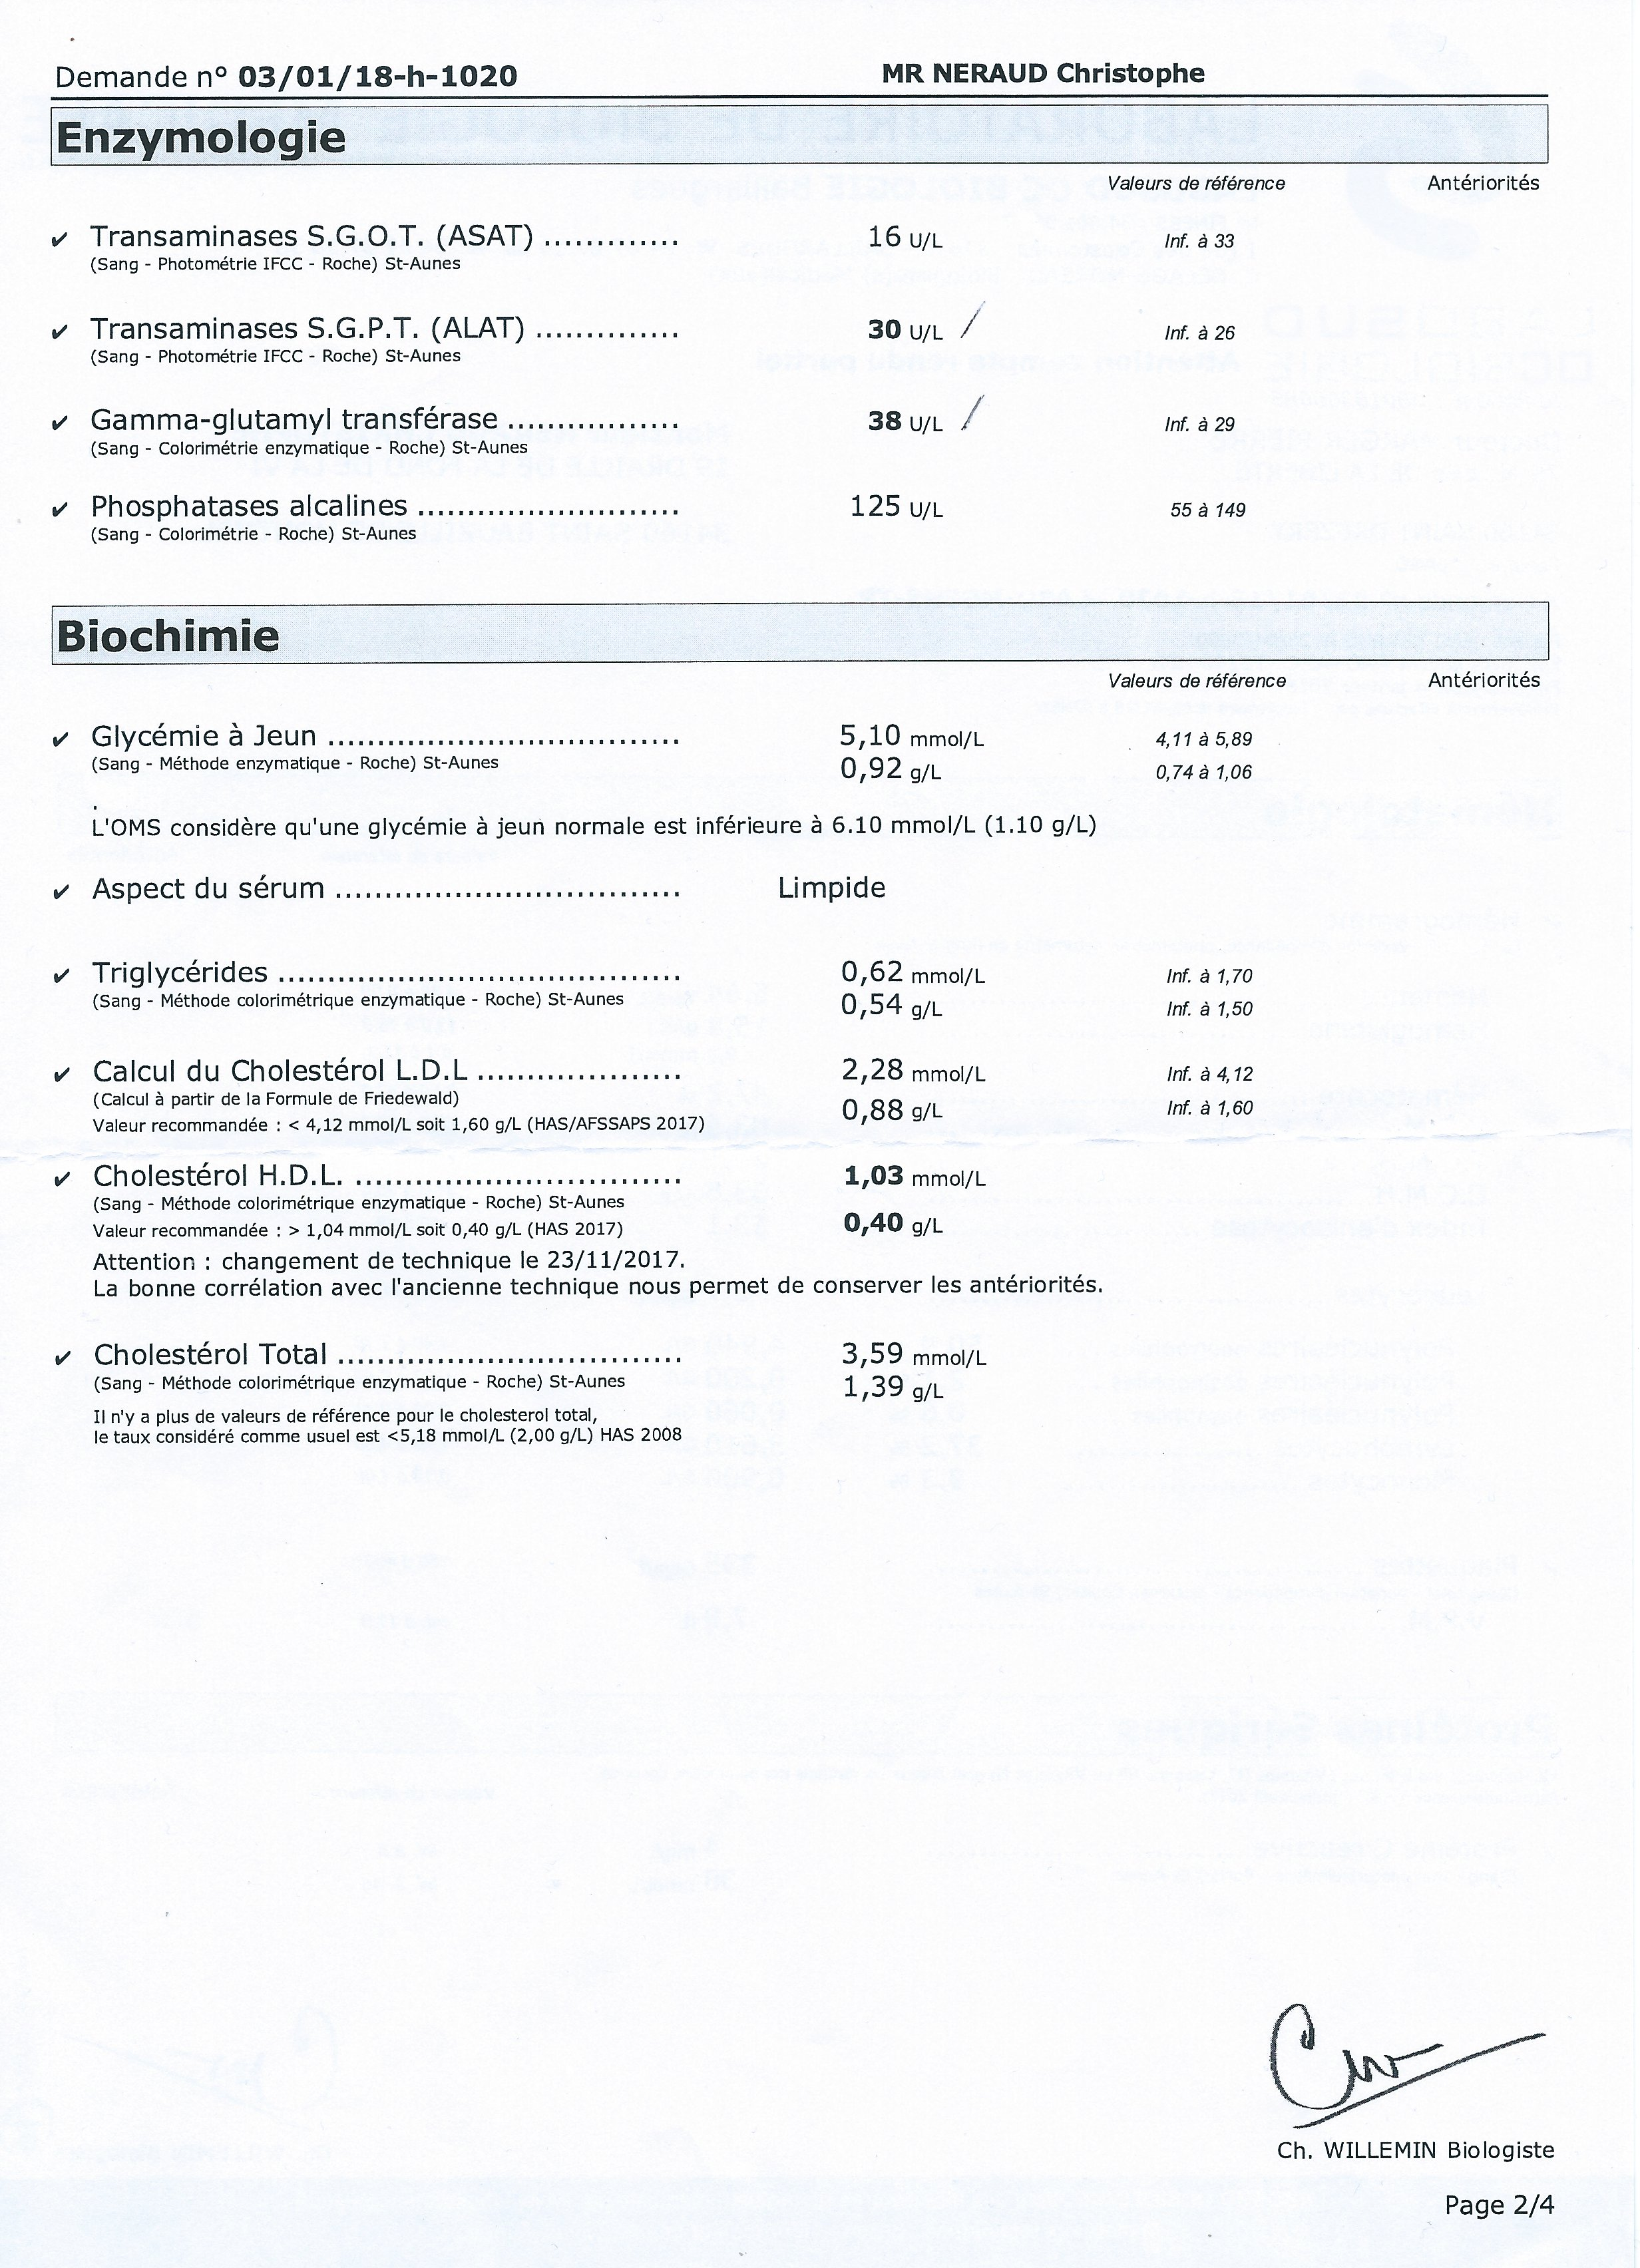
\includegraphics[scale=0.79]{03-01-2018/p2.JPG}
		\end{center}
		\caption{03 janvier 2018 : page 2}
	\end{figure}
	
	\begin{figure}[!h]
		\begin{center}
		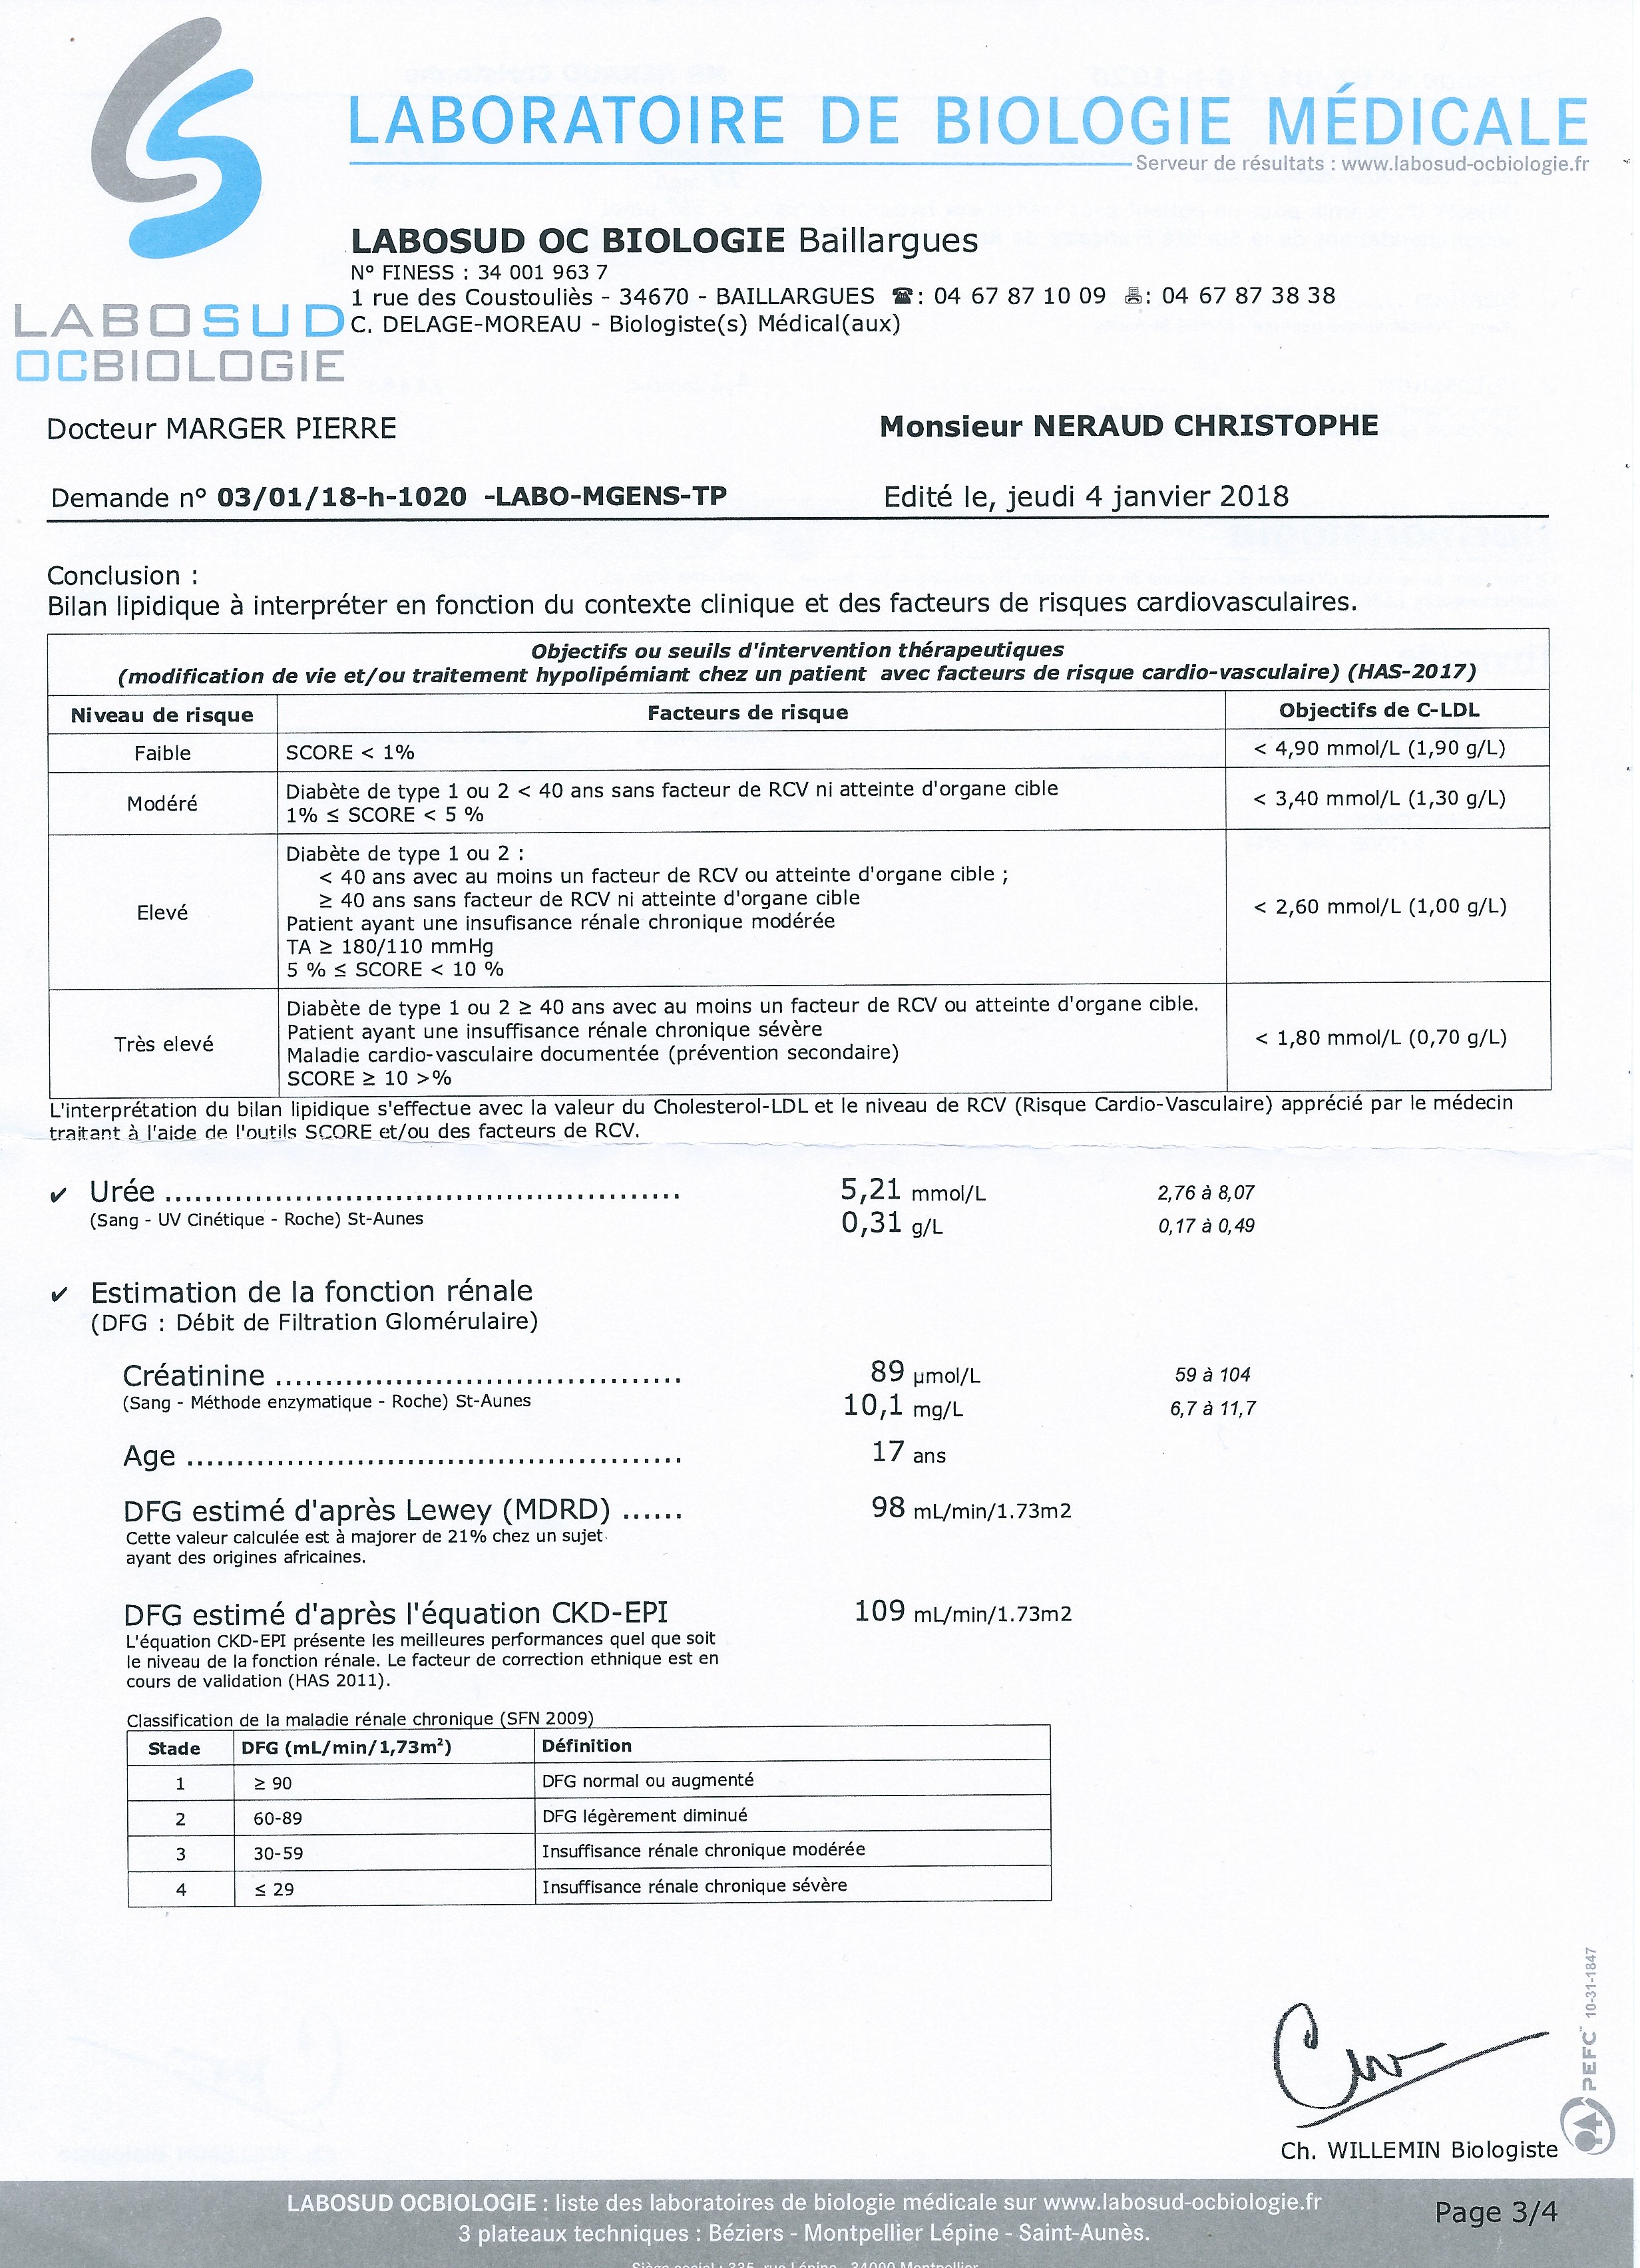
\includegraphics[scale=0.79]{03-01-2018/p3.JPG}
		\end{center}
		\caption{03 janvier 2018 : page 3}
	\end{figure}
	
	\begin{figure}[!h]
		\begin{center}
		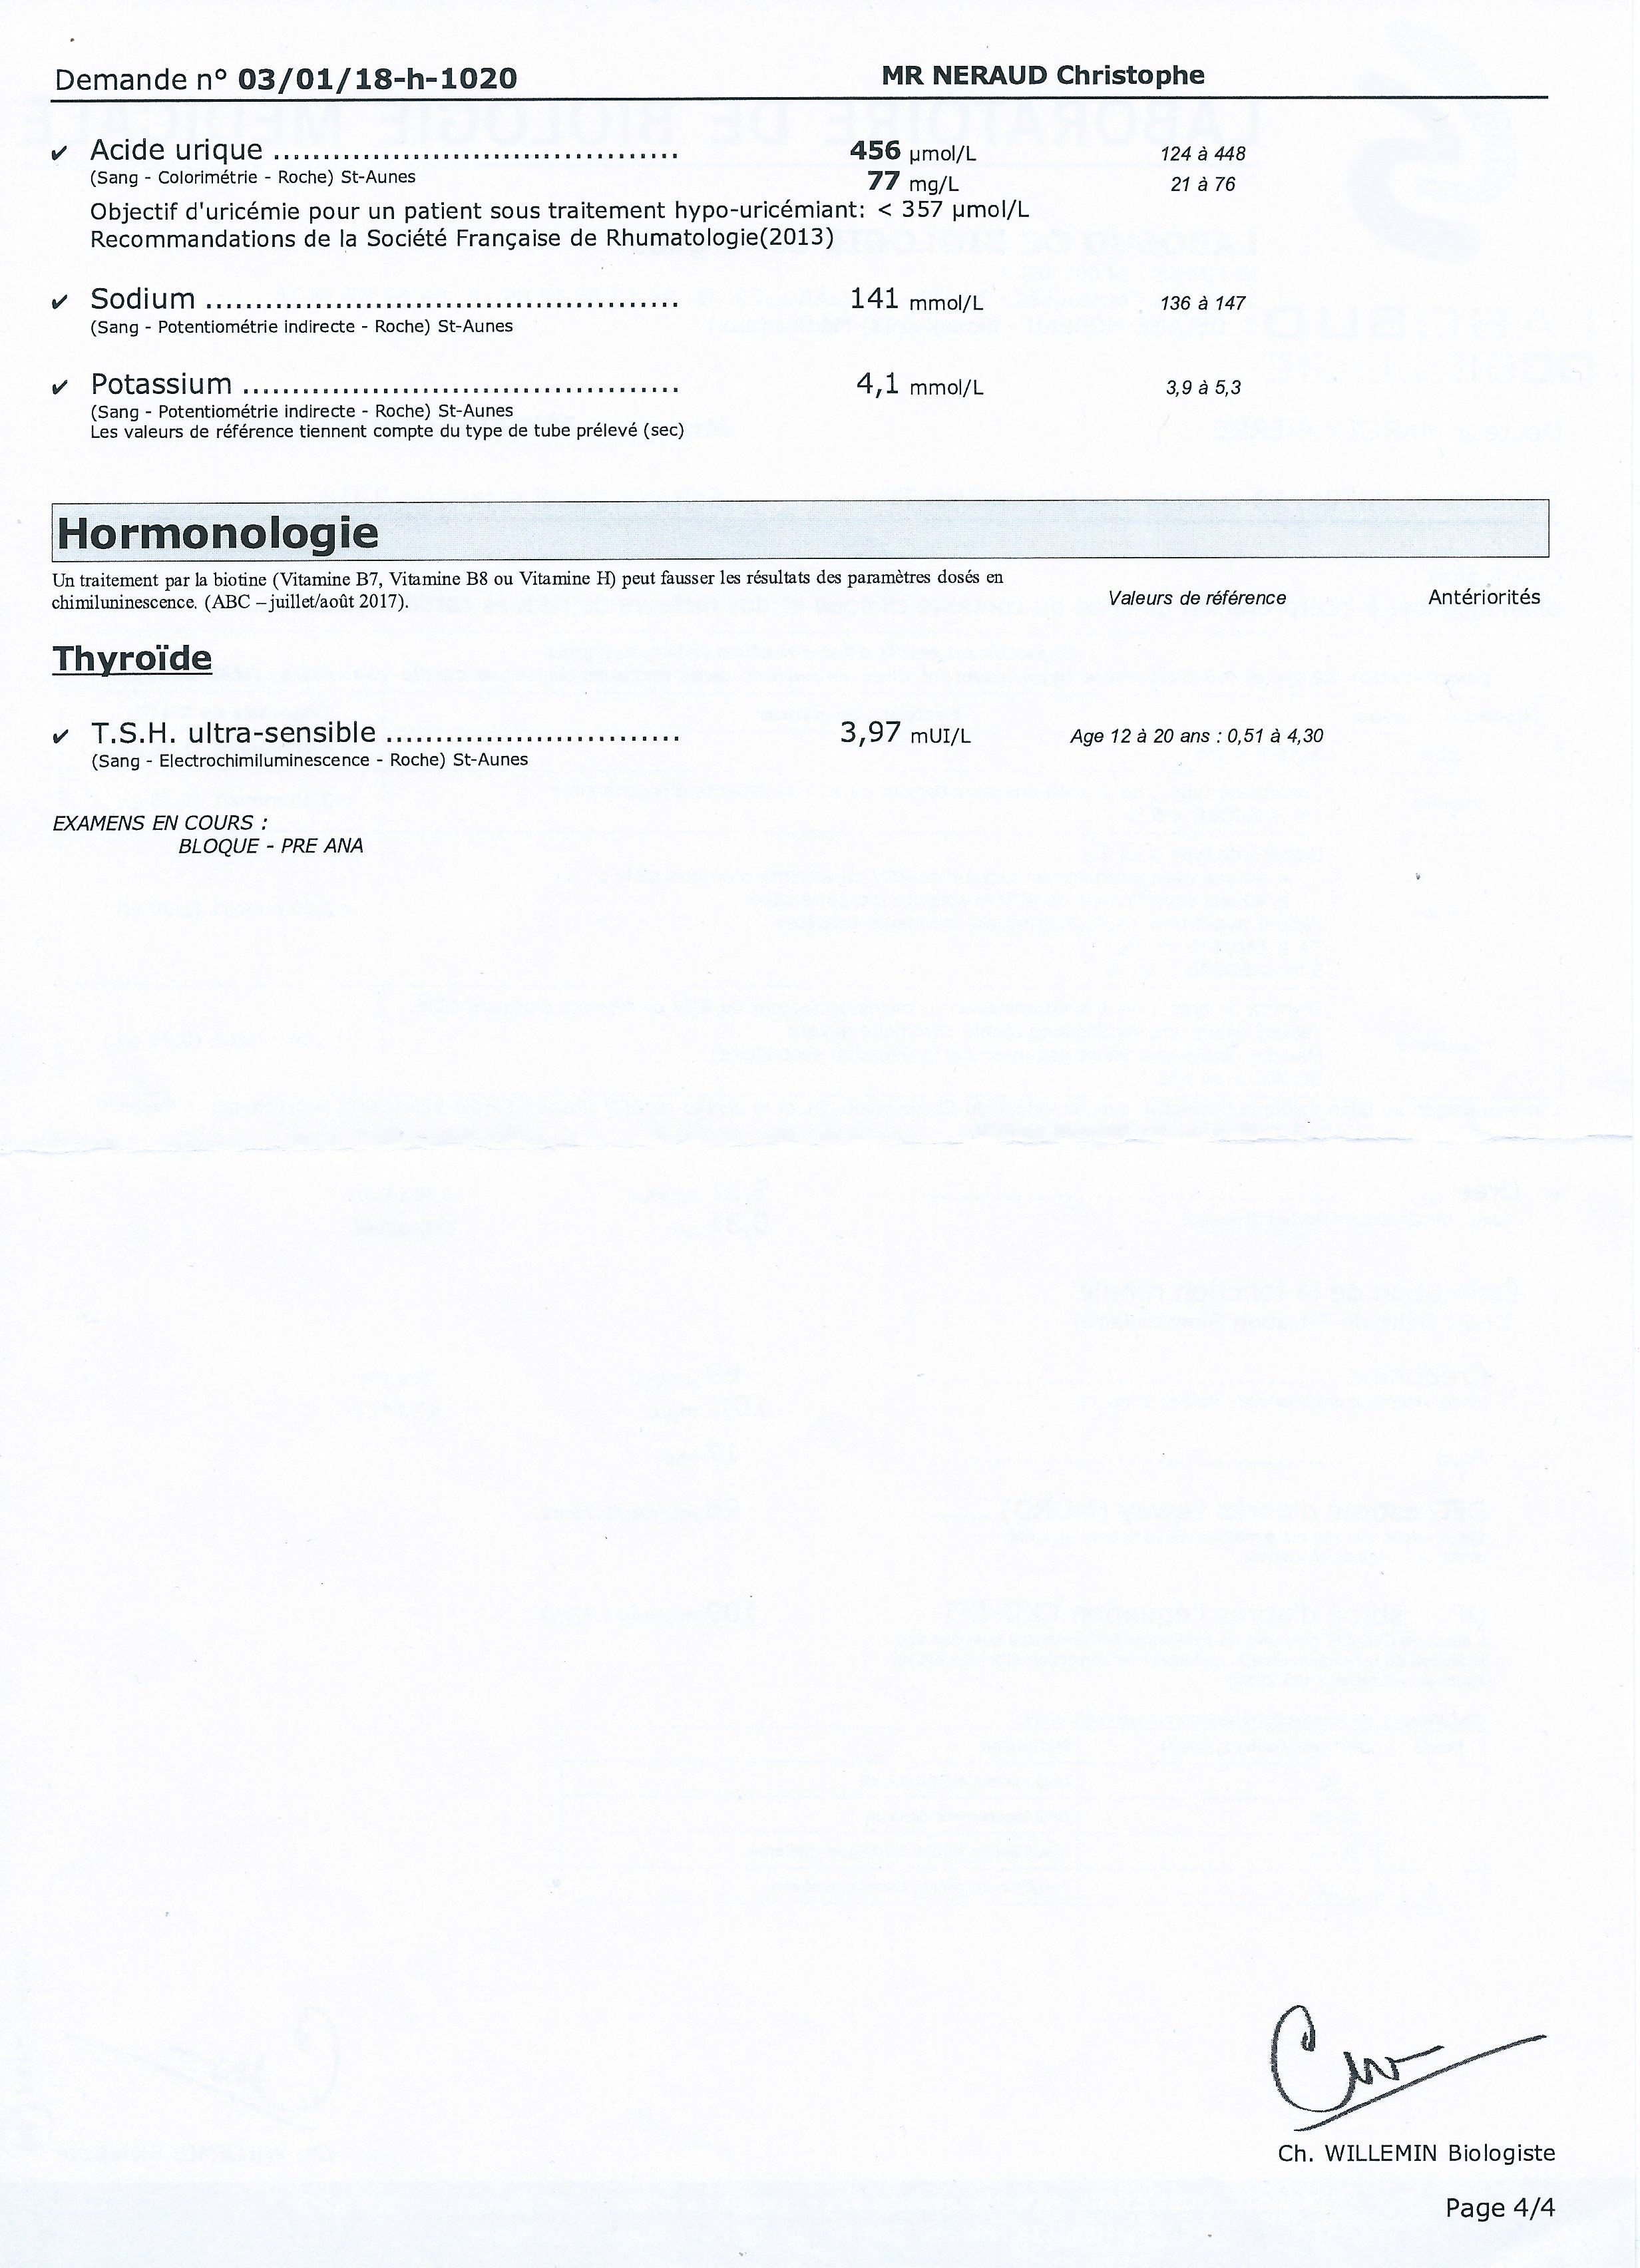
\includegraphics[scale=0.79]{03-01-2018/p4.JPG}
		\end{center}
		\caption{03 janvier 2018 : page 4}
	\end{figure}
	
\appendix
\section{Un mot sur les unités employées}
	En enzymologie, on exprime la quantité d'enzymes dans le sang en U$/$L, où U est l'unité enzymatique. C'est une unité d'activité enzymatique représentant la quantité d'enzyme nécessaire pour traiter une micromole de substrat en une minute dans des conditions opératoires qui doivent être précisées avec la mesure (pH, température, paramètres de solution). L'unité enzymatique n'est pas une unité du système international, mais y est liée par le \textit{katal}, qui lui est dans le système international. On retiendra : $1 \;\mathrm{kat} = 6 \cdot 10^7$ U. Cette unité correspond à des mol $\cdot$ s $^{-1}$.
	

\printindex

\listoffigures
\end{document}

















